\section{Relato de Experiência}
\label{sec:estudo}

Foi aplicado um questionário na equipe de desenvolvimento do Novo Portal do Software Público, onde os mesmos poderiam expressar o quanto estão aprendendo com o projeto e o quanto o projeto está ajudando na sua formação.

O questioário foi respondido por 17 integrantes do projeto que têm entre 20 e 26 anos, os quais então entre o 5º e o 10º semestre do curso de Engenharia de Software.

A primeira questão pretendia averiguar o nível de conhecimento dos entrevistados, em uma escala de 1 a 5, em relação às ferramentas que estão sendo utilizadas no projeto. Como resultados tivemos que 63\% responderam nível 3, 19\% responderam nível 2 e 19\% responderam nível 4.

A segunda questão pretendia averiguar o quanto o projeto está contribuindo para a formação do entrevistado. Em uma escala de 0 a 5, 69\% dos entrevistados responderam "5 -Contribui muito, mais que determinadas disciplinas", 19\% dos entrevistados responderam "4 - Contribui, no mesmo nível de muitas disciplinas" e 13\% dos entrevistados responderam "3 - Contribui, da mesma forma que um estágio convencional".

\begin{figure}[htpb]
  \begin{center}
    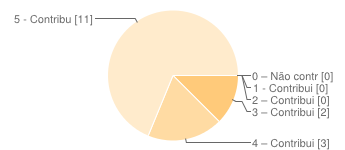
\includegraphics[width=.37\textwidth]{images/chart1.png}
  \end{center}
  \caption{Respostas do nível de contribuição do projeto na sua formação}
  \label{fig:core_concurrent}
\end{figure} 

A terceira questão está relacionada, também em uma escala de 0 a 5, a quanto o projeto atrapalha a sua performance nas disciplinas da graduação. Como resultados, 19\% dos entrevistados responderam "3 - Atrapalha minha graduação da mesma forma que um estágio", 50\% dos entrevistados responderam "2 - Atrapalha moderadamente", 19\% dos entrevistados responderam "1 - Atrapalha pouco, menos que um estágio" e 13\% dos entrevistados responderam "0  Não atrapalha em nada na minha graduação".

\begin{figure}[htpb]
  \begin{center}
    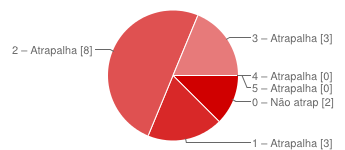
\includegraphics[width=.37\textwidth]{images/chart2.png}
  \end{center}
  \caption{Respostas do nível de performance nas disciplinas de graduação}
  \label{fig:core_concurrent}
\end{figure} 

A quarta questão averigua o quanto, em uma escala de 0 a 5, os conhecimentos adiquiridos durante a execução do projeto ajudam os entrevistados nas disciplinas da graduação. Como resultados, 7\% dos entrevistados responderam "5 - Ajuda muito, sempre utilizo os conhecimentos adiquiridos nas disciplinas da graduação	", 47\% respondeu "4  Ajuda muito, utilizo os conhecimentos com frequência nas disciplinas da graduação", 27\% respondeu "3 - Ajuda, utilizo os conhecimentos nas disciplinas da graduação" 13\% respondeu "2 - Ajuda moderadamente, as vezes utilizo os conhecimentos adquiridos no projeto" e 7\% respondeu "1 – Ajuda um pouco, utilizo pouco os conhecimentos do projeto".

\begin{figure}[htpb]
  \begin{center}
    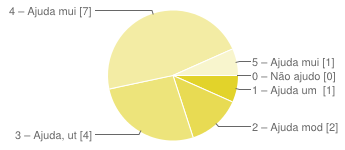
\includegraphics[width=.37\textwidth]{images/chart3.png}
  \end{center}
  \caption{Respostas do nível de conhecimento adquirido}
  \label{fig:core_concurrent}
\end{figure} 

E a quinta questão perguntou o quanto, em uma escala de 0 a 5, o entrevistado acredita que o projeto do Novo SPB vai contribuir em experiência para o mercado de trabalho. Como resultados, 38\% responderam "5  O projeto me tornará experiente para o mercado de trabalho", 38\% responderam "4 - O projeto me dará muita experiência para o mercado de trabalho" e 25\% responderam "3 - O projeto me dará uma boa experiência para o mercado de trabalho".

\begin{figure}[htpb]
  \begin{center}
    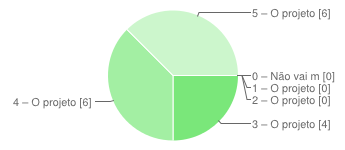
\includegraphics[width=.37\textwidth]{images/chart4.png}
  \end{center}
  \caption{Respostas do nível de experiência para o mercado de trabalho}
  \label{fig:core_concurrent}
\end{figure} 